\documentclass[12pt]{article}
\usepackage{geometry} % Pour passer au format A4
\geometry{hmargin=1cm, vmargin=1cm} % 

% Page et encodage
\usepackage[T1]{fontenc} % Use 8-bit encoding that has 256 glyphs
\usepackage[english,french]{babel} % Français et anglais
\usepackage[utf8]{inputenc} 

\usepackage{lmodern}
\setlength\parindent{0pt}

% Graphiques
\usepackage{graphicx,float,grffile}

% Maths et divers
\usepackage{amsmath,amsfonts,amssymb,amsthm,verbatim}
\usepackage{multicol,enumitem,url,eurosym,gensymb}

% Sections
\usepackage{sectsty} % Allows customizing section commands
\allsectionsfont{\centering \normalfont\scshape}

% Tête et pied de page
\usepackage{fancyhdr} 
\pagestyle{fancyplain} 
\fancyhead{} % No page header
\fancyfoot{}

% tikz pour les images
\usepackage{tikz}

\renewcommand{\headrulewidth}{0pt} % Remove header underlines
\renewcommand{\footrulewidth}{0pt} % Remove footer underlines

\newcommand{\horrule}[1]{\rule{\linewidth}{#1}} % Create horizontal rule command with 1 argument of height

%----------------------------------------------------------------------------------------
%	Début du document
%----------------------------------------------------------------------------------------

\begin{document}

%----------------------------------------------------------------------------------------
% RE-DEFINITION
%----------------------------------------------------------------------------------------
% MATHS
%-----------

\newtheorem{Definition}{Définition}
\newtheorem{Theorem}{Théorème}
\newtheorem{Proposition}{Propriété}

% MATHS
%-----------
\renewcommand{\labelitemi}{$\bullet$}
\renewcommand{\labelitemii}{$\circ$}
%----------------------------------------------------------------------------------------
%	Titre
%----------------------------------------------------------------------------------------

\setlength{\columnseprule}{1pt}

\section*{ie 3 - Trigonométrie}
\begin{center}
  \textit{Vincent Van Gogh - La normalité est une route pavée : on y marche aisément mais les fleurs n’y poussent pas.}
\end{center}
\horrule{2px}

\subsection*{Ex1 - Restituer}

\textbf{Restituer} les côtés : hypoténuse (HYP), adjacent (ADJ) et opposé (OPP) dans chacun des triangles suivants.

\begin{figure}[H]
  \centering
  
\includegraphics[width=0.6 \linewidth]{4x2-trigonometrie/sources/trigo-ex1a.pdf}
\end{figure}



\subsection*{Ex2 - Restituer}

\textbf{Restituer} les trois relations trigonométriques sinus (sin), cosinus (cos) et tangente (tan) en fonction des côtés Hypoténuse (HYP), Adjacent (ADJ) et Opposé (OPP). Ecrivez également la phrase \textit{mémoire} qui permet de s'en rappeler. N'oubliez pas de citer la condition pour utiliser la trigonométrie dans un triangle.

\subsection*{Ex3 - Restituer}

\begin{multicols}{2}

  Dans les deux triangles suivants, \textbf{restituer} les trois relations trigonométriques sinus (sin), cosinus (cos) et tangente (tan) en fonction des côtés.

  \begin{figure}[H]
    \centering
    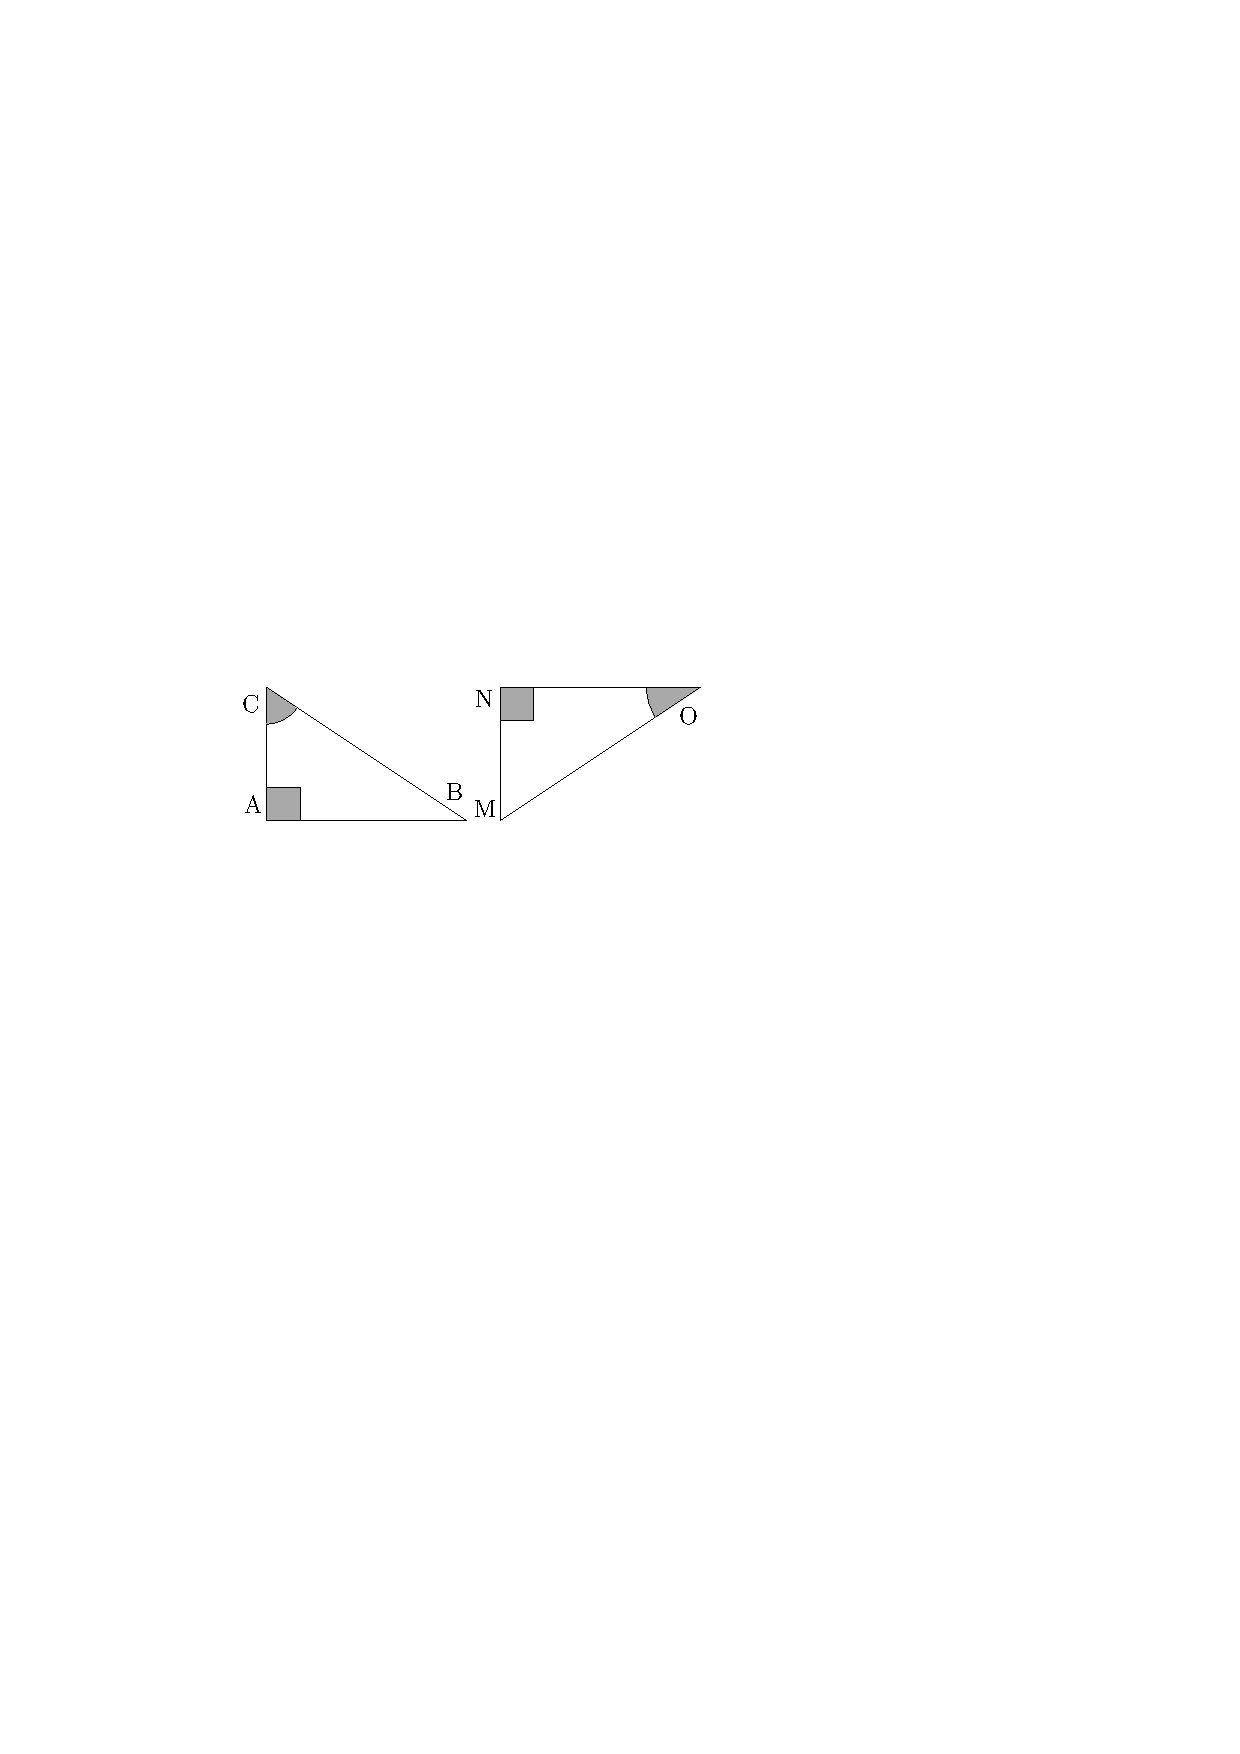
\includegraphics[width=0.6 \linewidth]{4x2-trigonometrie/sources/trigo-ex3a.pdf}
  \end{figure}
\end{multicols}

\subsection*{Ex4 - Modéliser}

\textbf{Modéliser} si on doit utiliser sinus (sin), cosinus (cos) ou tangente (tan). \textbf{Justifier} en écrivant la formule trigonométrique qui relie l'angle aux côtés.

\begin{figure}[H]
  \centering
  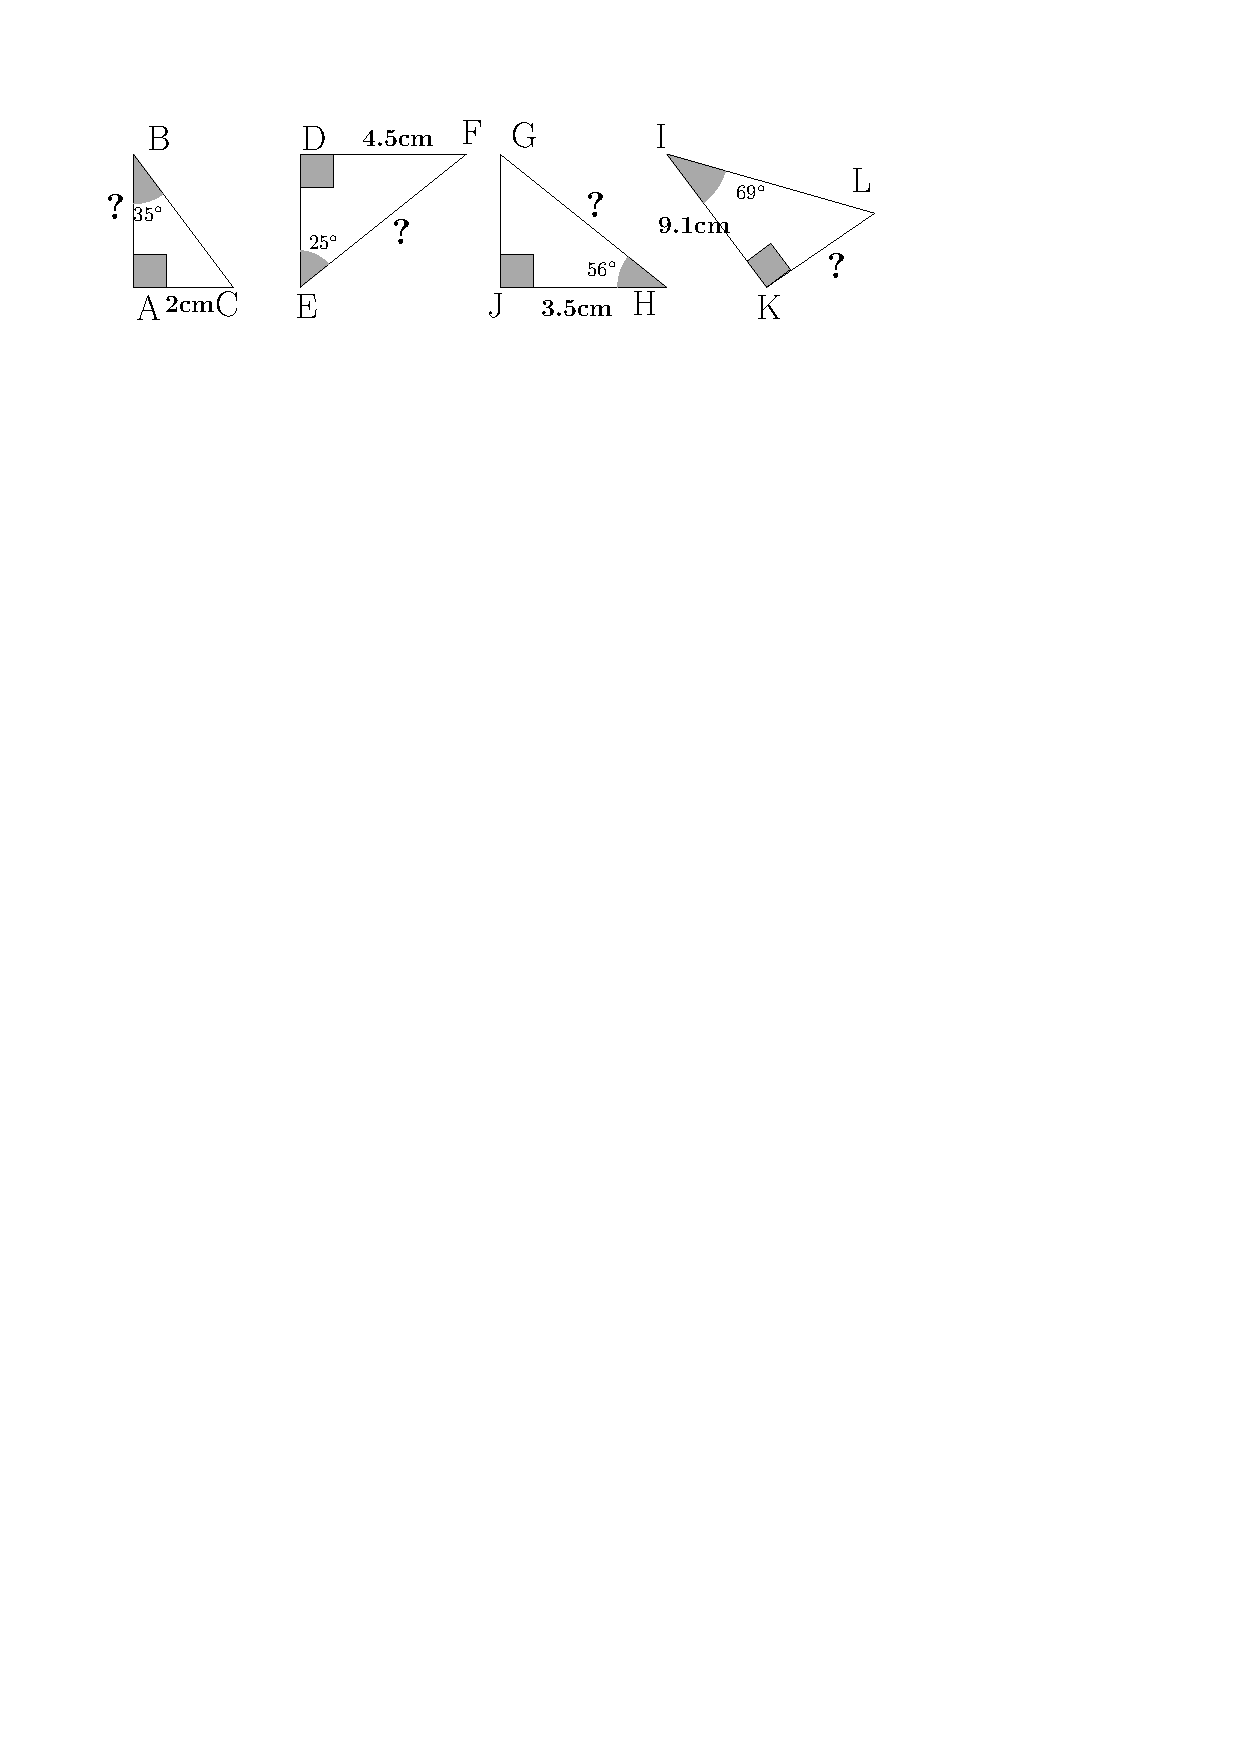
\includegraphics[width=0.6 \linewidth]{4x2-trigonometrie/sources/trigo-ex4a.pdf}
\end{figure}


\subsection*{Ex5 - Calculer}

\textbf{Calculer} à l'aide de la calculatrice et remplir le tableau. Mettre une valeur approchée arrondie à deux chiffres après la virgule. 

\begin{center}
  \begin{tabular}{| c || c | c | c |  c |  c |  c|}
    \hline
    &  12\degree & 22\degree & 45\degree & 62\degree & 82\degree & 90\degree \\
    \hline
    sin & \hspace{1.5cm} &  \hspace{1.5cm} &  \hspace{1.5cm} &  \hspace{1.5cm} &  \hspace{1.5cm} & \hspace{1.5cm} \\
    \hline
    cos & & & & & &  \\
    \hline
    tan  & & & & & &  \\
    \hline
  \end{tabular}
\end{center}

\newpage

\section*{ie 3 - Trigonométrie}
\begin{center}
  \textit{Vincent Van Gogh - La normalité est une route pavée : on y marche aisément mais les fleurs n’y poussent pas.}
\end{center}
\horrule{2px}

\subsection*{Ex1 - Restituer}

\textbf{Restituer} les côtés : hypoténuse (HYP), adjacent (ADJ) et opposé (OPP) dans chacun des triangles suivants.

\begin{figure}[H]
  \centering
  
\includegraphics[width=0.6 \linewidth]{4x2-trigonometrie/sources/trigo-ex1b.pdf}
\end{figure}



\subsection*{Ex2 - Restituer}

\textbf{Restituer} les trois relations trigonométriques sinus (sin), cosinus (cos) et tangente (tan) en fonction des côtés Hypoténuse (HYP), Adjacent (ADJ) et Opposé (OPP). Ecrivez également la phrase \textit{mémoire} qui permet de s'en rappeler. N'oubliez pas de citer la condition pour utiliser la trigonométrie dans un triangle.

\subsection*{Ex3 - Restituer}

\begin{multicols}{2}

  Dans les deux triangles suivants, \textbf{restituer} les trois relations trigonométriques sinus (sin), cosinus (cos) et tangente (tan) en fonction des côtés.

  \begin{figure}[H]
    \centering
    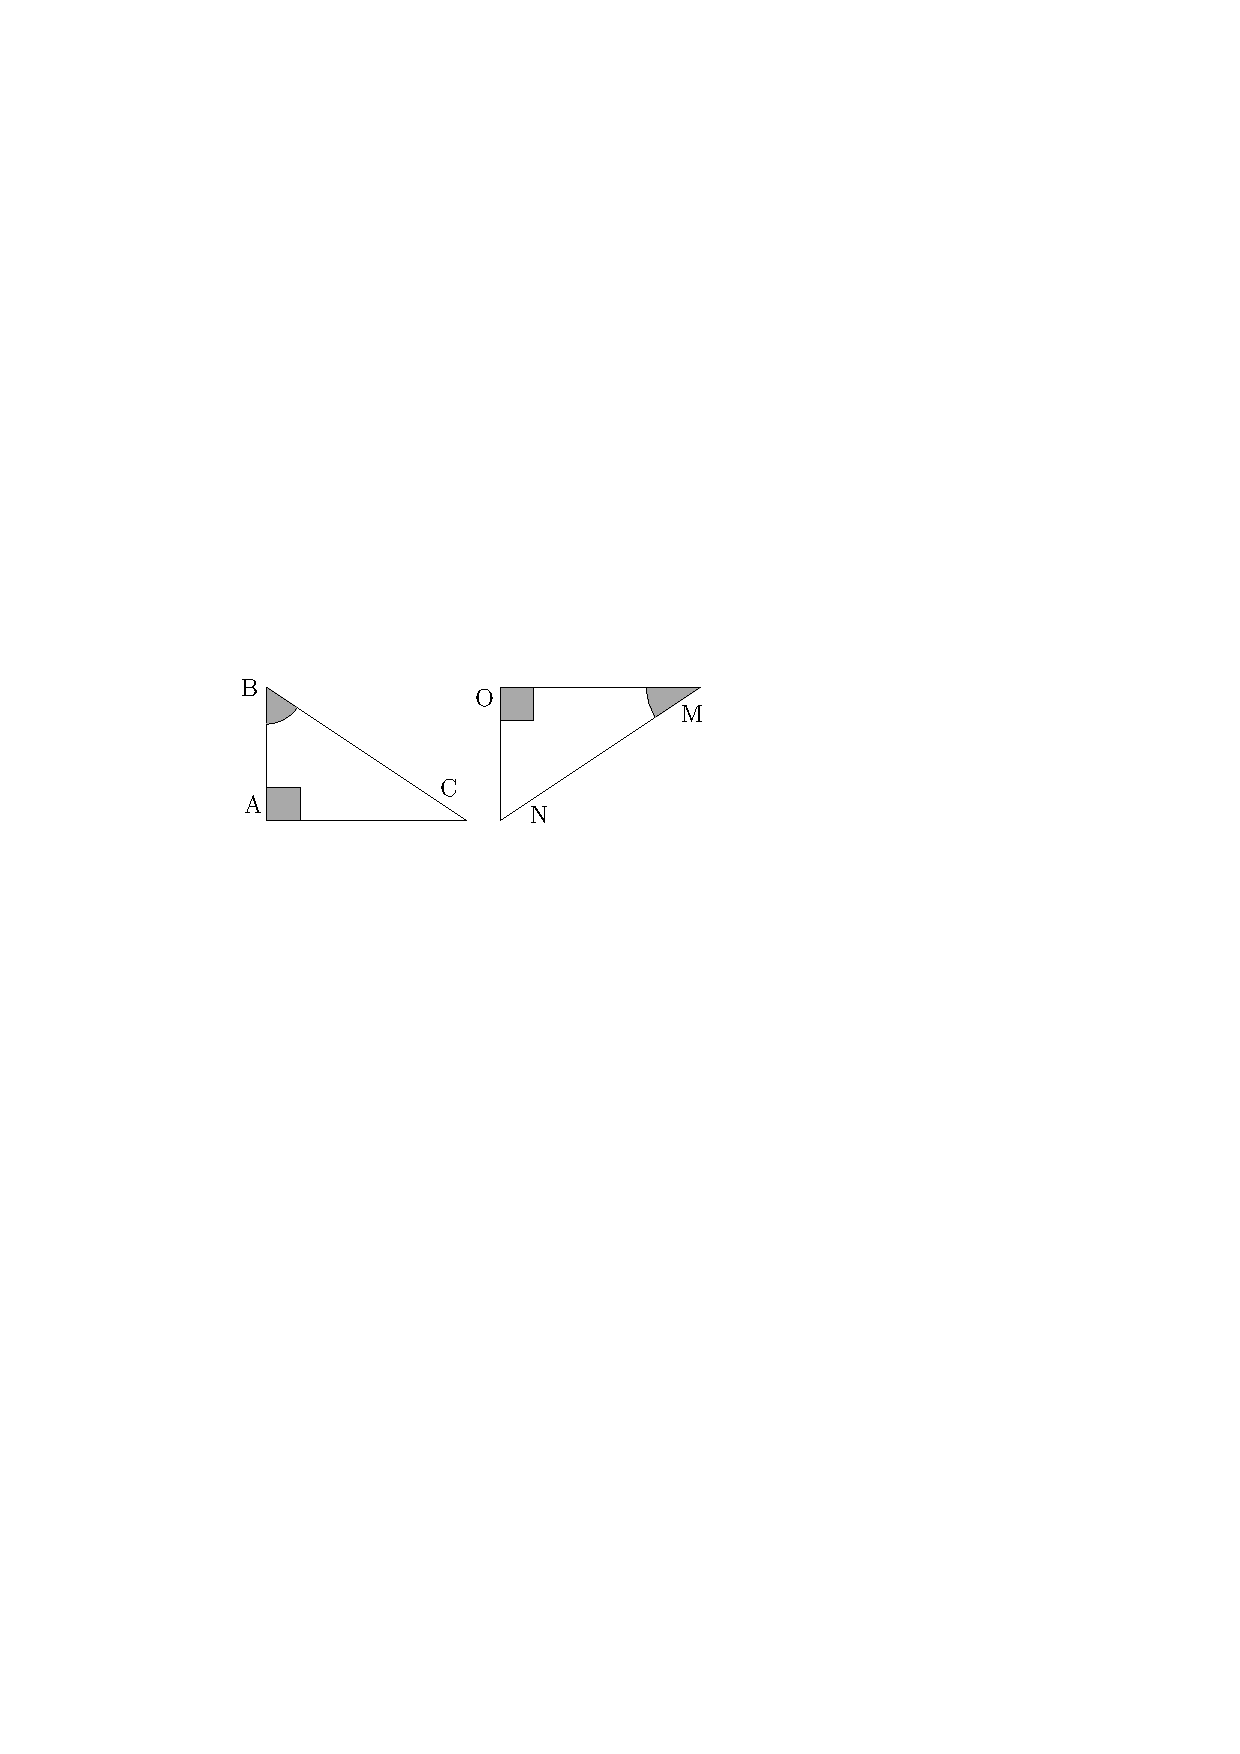
\includegraphics[width=0.6 \linewidth]{4x2-trigonometrie/sources/trigo-ex3b.pdf}
  \end{figure}
\end{multicols}

\subsection*{Ex4 - Modéliser}

\textbf{Modéliser} si on doit utiliser sinus (sin), cosinus (cos) ou tangente (tan). \textbf{Justifier} en écrivant la formule trigonométrique qui relie l'angle aux côtés.

\begin{figure}[H]
  \centering
  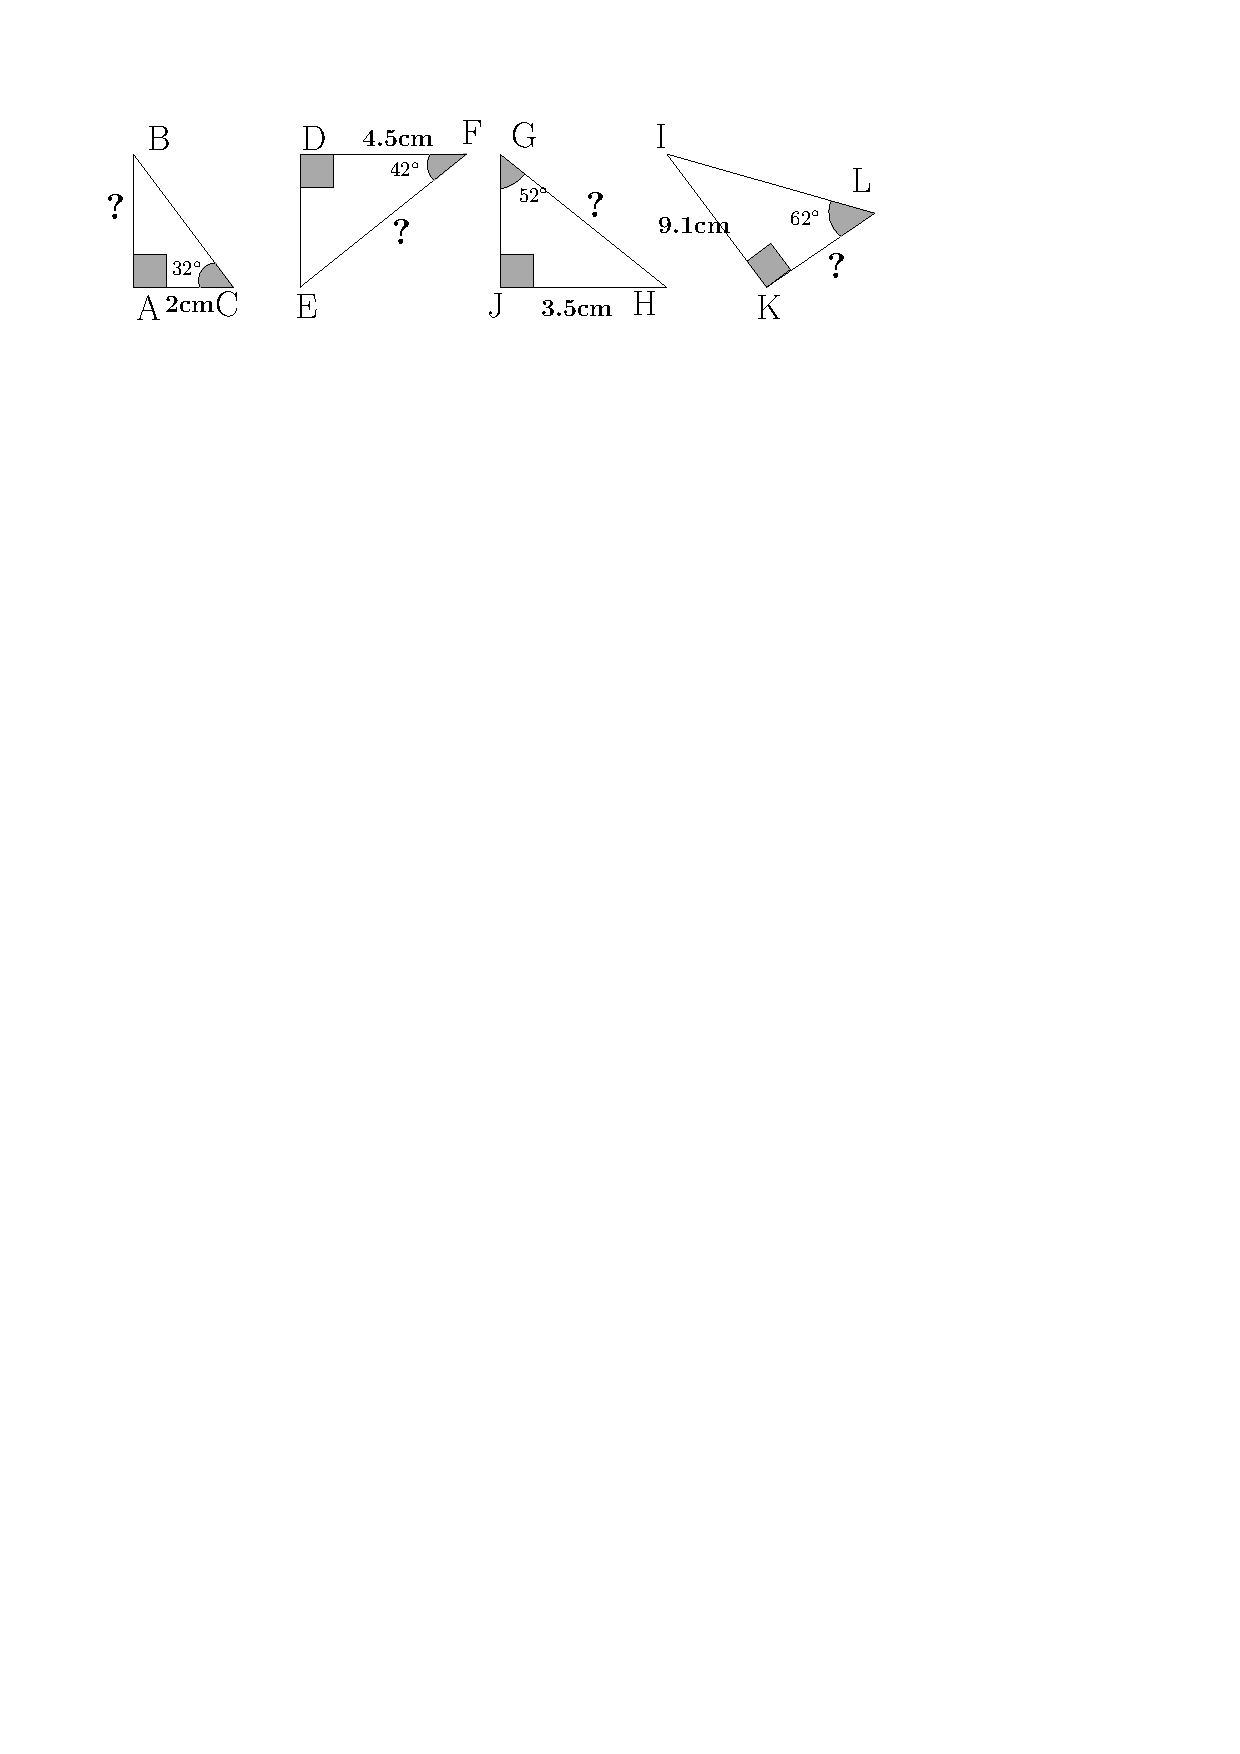
\includegraphics[width=0.6 \linewidth]{4x2-trigonometrie/sources/trigo-ex4b.pdf}
\end{figure}


\subsection*{Ex5 - Calculer}

\textbf{Calculer} à l'aide de la calculatrice et remplir le tableau. Mettre une valeur approchée arrondie à deux chiffres après la virgule. 

\begin{center}
  \begin{tabular}{| c || c | c | c |  c |  c |  c|}
    \hline
    &  14\degree & 24\degree & 45\degree & 64\degree & 84\degree & 90\degree \\
    \hline
    sin & \hspace{1.5cm} &  \hspace{1.5cm} &  \hspace{1.5cm} &  \hspace{1.5cm} &  \hspace{1.5cm} & \hspace{1.5cm} \\
    \hline
    cos & & & & & &  \\
    \hline
    tan  & & & & & &  \\
    \hline
  \end{tabular}
\end{center}


\end{document}
